\documentclass[a4paper]{llncs}
\usepackage[plain]{algorithm}
\usepackage{algpseudocode}
\usepackage{amsmath}
\usepackage{dcolumn}
\usepackage{tikz}
\usepackage{float}
\usepackage{hyperref}
\usetikzlibrary{positioning}
\usetikzlibrary{calc}
\usetikzlibrary{arrows,shapes,backgrounds}
\usetikzlibrary{shadows}

\newcommand{\eg}{\textit{e.g.}}

\renewcommand{\a}[1]{\v{a}_{#1}}
\renewcommand{\L}{\mathcal{L}}
\renewcommand{\v}[1]{\vec{#1}}
\newcommand{\av}[1]{\langle#1\rangle}
\newcommand{\vphi}{\varphi}
\newcommand{\vi}{{\vec{i}}}
\newcommand{\vj}{{\vec{j}}}
\newcommand{\vmu}{\vec{\mu}}
\newcommand{\ie}{{\textit{i.e.}}}
\newcommand{\fillblockgray}[2]{
\pgfmathtruncatemacro\llx{\bksize*(#1)-2}
\pgfmathtruncatemacro\lly{\bksize*(#2)-2}
\pgfmathtruncatemacro\urx{\bksize*(#1+1)+1}
\pgfmathtruncatemacro\ury{\bksize*(#2+1)+1}
\foreach \x in {\llx, ..., \urx}
  \foreach \y in {\lly,...,\ury} {
    \fill[gray] (\x, \y) circle(.25);
  }
}

\newcommand{\npartition}[3]{
\pgfmathtruncatemacro\row{Mod(#2,4)}
\ifnum \row = 0
   \pgfmathtruncatemacro\num{Mod(#1,4)}
\else \ifnum \row  = 1
   \pgfmathtruncatemacro\num{Mod(#1,4)+4}
\else \ifnum \row  = 2
   \pgfmathtruncatemacro\num{Mod(Mod(#1,4)+2,4)}
\else \ifnum \row  = 3
   \pgfmathtruncatemacro\num{Mod(Mod(#1,4)+2,4)+4}
\fi
\fi
\fi
\fi
\ifnum \num = #3
\draw[draw=black,fill=red] (#1, #2) circle(0.4);
\fi

}

\newcommand{\markpartition}[3]{
\pgfmathtruncatemacro\llx{\bksize*(#1)}
\pgfmathtruncatemacro\lly{\bksize*(#2)}
\pgfmathtruncatemacro\urx{\bksize*(#1+1)-1}
\pgfmathtruncatemacro\ury{\bksize*(#2+1)-1}
\foreach \x in {\llx, ..., \urx}
  \foreach \y in {\lly,...,\ury} {
    \npartition{\x}{\y}{#3}
  }
}

\definecolor{colorone}{HTML}{777777} % default 116699
\definecolor{colortwo}{HTML}{DDDDDD} % default CCCCCC
\def\bksize{8}
\def\bkcount{4}
\def\lcsize{5}

%%%%%%%%%%%%%%%%%%%%%%%%%%%%%%%%%%%%%%%%%%%%%%%%%%%%%%%%%%%%%%%%%%%%%%%%%%%%%%%%

\title{ GPU-accelerated and CPU SIMD Optimized \\
  Monte Carlo Simulation of $\phi^4$ Model } \author{ Piotr
  Bialas\inst{1}\inst{2}\thanks{\email{pbialas@th.if.uj.edu.pl}} \and
  Jakub Kowal\inst{1}\thanks{\email{jakub.kowal@uj.edu.pl}} \and Adam
  Strzelecki\inst{1}\thanks{\email{adam.strzelecki@uj.edu.pl}} }
\institute{ Faculty of Physics, Astronomy and Applied Computer Science \\
  Jagiellonian University ul. Reymonta 4, 30-059 Krakow, Poland
  \and Mark Kac Complex Systems Research Centre \\
  Faculty of Physics, Astronomy and Applied Computer Science \\
  Jagiellonian University, Reymonta 4, 30-059 Krakow, Poland }

\begin{document}

\maketitle

\begin{abstract}
  In this contribution we describe an efficient GPU implementation of
  the Monte-Carlo simulation of the Ginzburg--Landau model.  We
  achieve the performance close to
  50\% of the peak performance of the used GPU. We compare
  this performance with a parallelized and vectorized CPU code and
  discuss the observed differences.
\end{abstract}

Keywords: GPU computing, vectorization. Monte-Carlo simulations.

%%%%%%%%%%%%%%%%%%%%%%%%%%%%%%%%%%%%%%%%%%%%%%%%%%%%%%%%%%%%%%%%%%%%%%%%%%%%%%%%

\section{Introduction}

The Graphical Processing Units (GPU) emerge these days as the most efficient
devices for numerical calculations. To ascertain this it is sufficient to look
at the list of 500 supercomputers\cite{top500} and count how many of them have
GPU accelerators and this trend is still increasing. This was made possible not
only by the accessibility of the hardware but also by the realization from the
side of the vendors that those units can be used also for computations, and
providing user with suitable software interface to do this. Technologies like
CUDA and OpenCL make the GPU relatively easy accessible to C/C++ programmers.
In the meantime also most of the numerical packages vendors have added GPU
support to their tools.

However like with most of the computer languages there is a learning gap
between using them and using them efficiently. The GPU are not only {\em
massively parallel} machines but essentially {\em vector machines}. This is a
trend visible also in the CPU market: the SSE extensions introduced four floats
wide vector (SIMD) instructions, AVX eight floats wide and \emph{Xeon Phi} 16
floats wide\footnote{The \emph{Xeon Phi} strictly speaking is not a CPU but an
accelerator. However its cores are based on \emph{Intel} \emph{Pentium} CPU
micro-architecture.}. To get most out of the hardware it is crucial to
vectorize the algorithm and make good use of the available memory hierarchy.

In this contribution we present an efficient implementation, both on GPU and
CPU, of the Monte-Carlo simulations of the discretized version of the
Ginzburg--Landau model. The Ginzburg-Landau model is probably after the Ising
model the second most important model of the statistical physics (for an
excellent introduction to those topics see \cite{binney}). It is the basis for
the modern theory of the phase transitions. Under the name of the $\phi^4$
theory it is a model for the scalar field that describes among other things the
much publicized lately Higgs particle. It is a simple model to formulate, but
in spite of its simplicity unsolvable. While many approximate methods exists to
study its properties Monte-Carlo simulations are used extensively and their
importance is growing as the speed and the accessibility of the new fast
hardware increases.

Our motivation was to develop a tool to accompany the lecture on Statistical
Field Theory given by one of the authors. The idea was to create a kind of
``virtual lab'' where students could study the effects of various parameters on
the properties of the model. This requires a fast implementation working on the
easily accessible commodity hardware, so the results can be obtained in
reasonably short time. For the educational reasons we also included a
``cut-off'' term (see next section) in the model, which while not strictly
necessary allows for greater clarity of the presentation. This term however
introduces the interactions between the sites that are not nearest neighbors
(see figure~\ref{fig:nn}) complicating the parallelization of the algorithm. We
have obtained a hundredfold speedup compared with our old CPU version. That
drew our attention to the inefficiency of the CPU code. We have completely
rewritten the code taking advantage of the many cores and SIMD instructions of
the CPU, paradoxically it took more effort than implementing the GPU version.

We believe however that our contribution is relevant to a wider audience.
Monte-Carlo simulations of this type play an important role in statistical
physics, solid state physics and field theory. Those simulations are usually
very time consuming so the speed of the algorithm is of a paramount importance.
Our implementation can be easily adapted to many variants of the model as we
describe in more detail later. The GPU implementation is targeted for small
desktop machines with commodity CUDA enabled graphics cards and is up to 25
times faster than CPU program running on the same machine. Such ``small-scale''
computing plays a very important role in science as it provides for fast
feedback right at the workplace, without resorting to more laborious and/or
expensive bigger machines.

Apart from providing ready to use code, which will be available online, we hope
to contribute also to general methodology of adapting Monte-Carlo to SIMD
architectures. This clearly is a trend in modern hardware but much of the
knowledge remains tacit in nature. We have found two published GPU
implementations of similar model, however they were mainly discrete spin models
with nearest neighbor interactions\cite{spin1,spin2,weigel}. We use a
continuous field model with extended neighborhood that to our knowledge was not
yet ported to the GPU.

\section{Ginzburg--Landau model and Monte-Carlo simulations}

Ginzburg--Landau model that we use in its discretized form is defined by the
Hamiltonian\cite{parisi}:

\begin{equation*}\label{eq:hamiltonian}\begin{split}
H[\varphi]&=\sum_{\vi}\Biggl(
\frac{1}{2}\sum_{\mu=1}^d(\vphi(x_\vi+\a{\mu})-\vphi(x_\vi))^2\\
&\phantom{=\sum_{\vi}\bigl(}+\frac{\mu^2}{2}|\vphi(x_{\vi})|^2+
\frac{g}{24}(|\vphi(x_{\vi})|^2)^2\\
&\phantom{=\sum_{\vi}\bigl(}+
\frac{1}{2\Lambda}\Bigl(\sum_{\mu=1}^d
(\vphi(x_\vi+\a{\mu})-2\vphi(x_{\vi})+\vphi(x_\vi-\a\mu))\Bigr)^2\Biggr).
\end{split}
\end{equation*}

where $\vphi$ is a scalar\footnote{In general this can be a vector, but in this
contribution we restrict ourselves to scalar case.} field defined on the sites
of a $d$ dimensional lattice (we only consider $d=2$ and $3$). The $x_i$ denote
a site of the lattice where $i$ is a multidimensional index and $\a\mu$ denotes
the unit vector in the direction $\mu$. We use periodic boundary conditions \ie

\begin{equation}
\phi(x+L_{\mu}\a\mu)=\phi(x)
\end{equation}
where  $L_\mu$ is the number of lattice sites in direction $\mu$.
The Monte-Carlo simulations consist of
generating the field configurations with probability proportional to
$\exp(-H(\vphi))$.

The generation is done by the mean of the Metropolis
algorithm\cite{metropolis,binney}. This amounts to sequentially updating all
the points of the lattice. During each update we change the value of the field
$\vphi$ in on a single lattice point ($\vphi_i$ is a shorthand for
$\vphi(x_\vi)$).

\begin{equation}
\vphi_i\longrightarrow\widetilde{\vphi_i}=\vphi_i+\eta_i.
\end{equation}
The $\eta_i$ is a pseudo--random number drawn from a distribution such
that $P(\eta_i) = P(-\eta_i)$. In practice we draw  $\eta$ from the
uniform distribution on interval $[-\varepsilon,\varepsilon)$.  Then we
calculate the difference of the Hamiltonian's
\begin{equation}
\Delta H=H[\widetilde{\vphi_i}]-H[\vphi_i].
\end{equation}

If $\Delta H < 0$ we accept the change and substitute
$\widetilde{\vphi_i}$ for $\vphi_i$, otherwise we accept the change
with the probability $\exp(-\Delta H)$. In other words if we denote by
$P(\phi_i\rightarrow\phi_i+\eta_i)$ the probability of updating the
field at lattice site $x_i$ then it is given by
\begin{equation}
P(\vphi_i\rightarrow\vphi_i+\eta_i)=\min\left(1,\exp(-\Delta H)\right).
\end{equation}

The crucial feature of this algorithm is that the update is local {\em
  i.e.} $\Delta H$ depends only on the values of fields in the
immediate neighborhood of the updated point
\begin{equation}
\begin{split}
\Delta H & = -(\widetilde{\vphi_i}-\vphi_i)\, c_i\\
&\phantom{= -}
+(\widetilde{\vphi}^2_i-\vphi_i^2)\left(d+\frac{\mu^2}{2}+d (1+2d)\frac{1}{\Lambda}\right)\\
&\phantom{= -}+\frac{g}{4!}\left(\widetilde{\vphi}^4_i-\vphi^4_i\right)
\end{split}
\end{equation}
where
\begin{equation}
c_i=\left(c^{01}_i-\frac{1}{\Lambda}(c^{02}_i-4 d c^{01}_i+2 c^{11}_i )\right)
\end{equation}
and
\begin{equation}\label{eq:corona-terms}\begin{split}
c_i^{01}&=\sum_{\mu=1}^d\left(\vphi(x_\vi+\a\mu)+\vphi(x_\vi-\a\mu)\right)\\
c_i^{02}&=\sum_{\mu=1}^d\left(\vphi(x_\vi+2\a\mu)+\vphi(x_\vi-2\a\mu)\right)\\
c_i^{11}&=\sum_{\mu=}^d\sum_{\nu=1}^{\mu-1}
\bigl(\vphi(x_\vi+\a\mu+\a\nu)+\vphi(x_\vi-\a\mu-\a\nu)\\
&\phantom{+=\sum_{\mu=}^d\sum_{\nu=1}^{\mu-1}
}
+ \vphi(x_\vi+\a\mu-\a\nu)+\vphi(x_\vi-\a\mu+\a\nu)
\bigr)
\end{split}
\end{equation}

The term $c_i$ is referred to as \emph{corona} of the site $x_i$. The corona is
a weighted sum of the values of the field $\phi$ on the sites in the
neighborhood of the site $x_i$. Figure~\ref{fig:nn} provides a geometrical
interpretation of corona in two dimensions. In our case, because of the last
term in \eqref{eq:hamiltonian}, the corona is extended as compared to more
commonly used nearest neighbors neighborhood (squares on the
figure~\ref{fig:nn}). As we will show in the next section this considerably
complicates the parallelization of the algorithm.

\begin{figure}[H]
\begin{center}
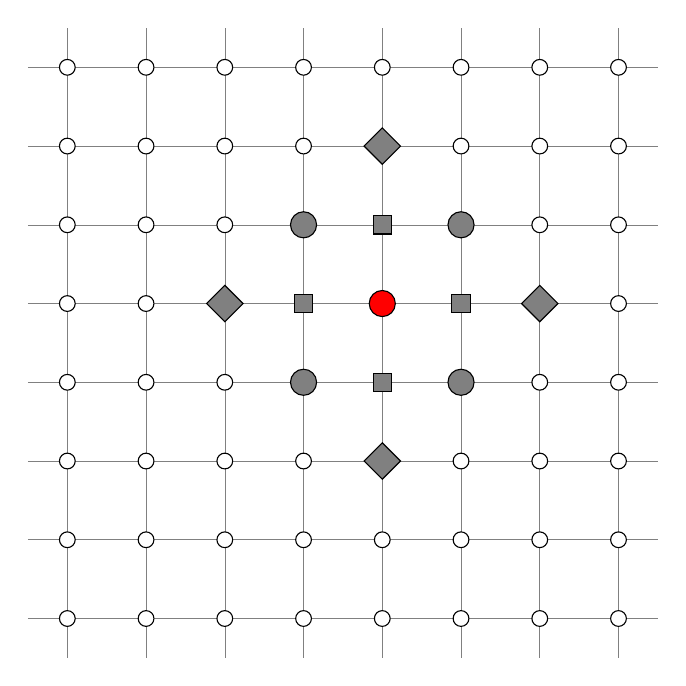
\begin{tikzpicture}
\def\lcsize{8}
\pgfmathtruncatemacro\lcsizem{\lcsize - 1}
\pgfmathtruncatemacro\lcsizeb{\lcsize - \bksize}
\pgfmathtruncatemacro\bksizea{\bksize - 2}
\pgfmathtruncatemacro\bksizeb{\bksize - 1}
\pgfmathtruncatemacro\bksizec{\bksize * 2}
\pgfmathtruncatemacro\bksizem{\bksizec - 1}
\pgfmathtruncatemacro\bksized{\bksizec + 1}

\draw[very thin, gray] (-.5, -.5) grid (\bksize - .5, \bksize - .5);

\foreach \x in {0,...,\lcsizem}
  \foreach \y in {0, ...,\lcsizem}
    \draw[fill=white,draw=black]  (\x, \y) circle[radius=0.1];

\coordinate (c) at (4,4);

\node at (c) [circle,fill=red,draw=black] {};

\def\coronaa{(0,1), (0,-1), (1,0), (-1,0)}
\def\coronab{(0,2), (0,-2), (2,0), (-2,0)}
\def\coronac{(1,1), (1,-1), (-1,-1), (-1,1)}

\foreach \p in \coronaa {
  \path (c) + \p node  [rectangle,fill=gray, draw=black] {};
}

\foreach \p in \coronab {
  \path (c) + \p node  [diamond,fill=gray,draw=black] {};
}
\foreach \p in \coronac {
  \path (c) + \p node  [circle,fill=gray, draw= black] {};
}
\end{tikzpicture}
\end{center}
\caption{\label{fig:nn}The neighborhood used to calculate the $\Delta
  H$. The values of the field $\phi$ on the gray marked lattice sites
  contribute to the corona $c_i$ with geometrical symbols marking the
  contribution to different terms: $c^{01}$ -- squares, $c^{11}$ --
  circles and $c^{02}$ -- diamonds.}
\end{figure}

%%%%%%%%%%%%%%%%%%%%%%%%%%%%%%%%%%%%%%%%%%%%%%%%%%%%%%%%%%%%%%%%%%%%%%%%%%%%%%%%

\section[gpu]{GPU implementation\footnote{Source code available at:
\url{https://github.com/ujhpc/phi4_cuda}}}

The Metropolis algorithm lends itself naturally to parallelization, however
some caution must be taken. Notably grid points that lie in the same
neighborhood cannot be updated together. That is if we update the red point on
the figure~\ref{fig:nn} we cannot update any of the gray points in the same
time. Basically this stems from the requirement that in order to process two
sites $x_a$ and $x_b$ in parallel those two operation must be independent. That
means that the joint probability
$P(\phi_a,\phi_b\rightarrow\phi_a+\eta_a,\phi_b+\eta_b)$ must factorize:

\begin{equation}
P(\phi_a,\phi_b\rightarrow\phi_a+\eta_a,\phi_b+\eta_b)
=P(\phi_a\rightarrow\phi_a+\eta_a)P(\phi_b\rightarrow\phi_b+\eta_b)
\end{equation}

This can be only achieved if $P(\phi_a\rightarrow\phi_a+\eta_a)$ does
not depend on the value of $\phi_b$ and vice versa.

To ensure that this condition is satisfied we decompose the lattice into
several sublattices such that points belonging to each sublattice are far
enough from each other and can safely be updated in parallel. In case of the
more commonly encountered nearest-neighbor interaction (squares on the
figure~\ref{fig:nn}) it is enough two divide the lattice in two sublattices by
labeling each side ``black'' or ``white'' as on the checkerboard (sometimes
this is also referred as ``even-odd'' decomposition)\cite{Checkboard}. It is
easy to see that no site has a nearest neighbor of the same color, so all the
sites of the same color can be updated in parallel. This would be the case of
the Ginzburg-Landau model without the last term in \eqref{eq:hamiltonian}.

As we consider in here a model with much bigger corona (see fig~\ref{fig:nn})
this simple decomposition is not sufficient any more. We have been unable to
find a decomposition requiring less then eight sublattices in two dimensions,
and 16 in three dimensions. The two dimensional decomposition is depicted on
the figure~\ref{fig:part} where we have marked each site (square) with the
index of the sublattice it belongs to.

\begin{figure}
\begin{center}
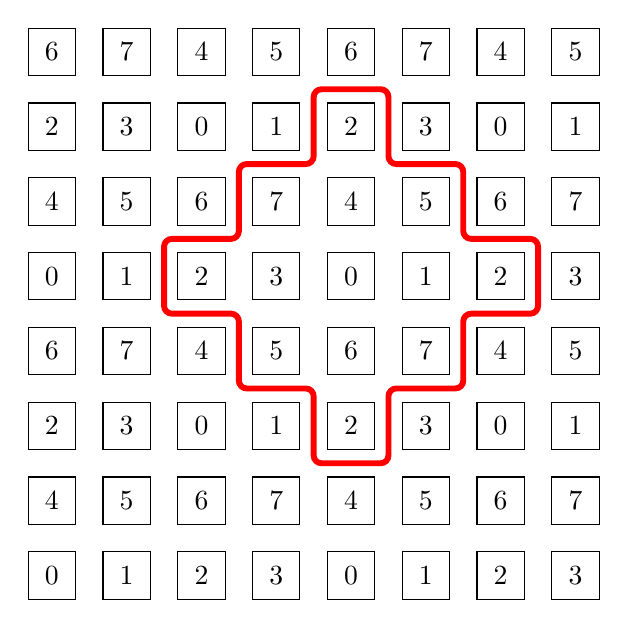
\begin{tikzpicture}[scale=0.95]

% \clip[rounded corners=0cm] (-1, -1) rectangle (\bksize + 1, \bksize + 1);

% \draw[help lines] (-1, -1) grid (\bksize + 1, \bksize + 1);

\pgfmathtruncatemacro\bksizem{\bksize - 1}

% % lattice points
 \foreach \x in {0, ..., \bksizem}
   \foreach \y in {0, ..., \bksizem} {
     \pgfmathtruncatemacro\four{Mod(\y,4)}
     \pgfmathtruncatemacro\eight{Mod(\x,4)+4*Mod(\y,2)}
     \ifnum \four<2
     \pgfmathtruncatemacro\eight{Mod(\x,4)+4*Mod(\y,2)}
     \node[draw,rectangle,minimum size=0.6cm] at (\x,\y)  {\eight};
     \else
     \pgfmathtruncatemacro\eight{Mod(\x+2,4)+4*Mod(\y,2)}
     \node[draw,rectangle,minimum size=0.6cm] at (\x,\y)  {\eight};
     \fi
}
% neighborhood
\def\neighborhood{--
  ++( 0,  -.5)-- ++( 1,  0)-- ++( 0, -.5 )-- ++(0, -.5)-- ++( 1, 0  )--
  ++( 0, -1.0)-- ++( 1,  0)-- ++( 0,  1.0)-- ++(1, 0  )-- ++( 0, 1.0)--
  ++( 1,  0  )-- ++( 0,  1)-- ++(-1,  0  )-- ++(0, 1  )-- ++(-1, 0  )--
  ++( 0,  1  )-- ++(-1,  0)-- ++( 0, -1  )--
  ++(-1,  0  )-- ++( 0, -1)-- ++(-1,  0  )-- ++(0, -.6)}

\pgfmathtruncatemacro\lchalf{\bksize / 2}

% main center neighborhood
\path[draw=red,  rounded corners=.1cm, shorten >=2pt, line width=.75mm]
(\lchalf - 2.5, \lchalf) \neighborhood;
\end{tikzpicture}
\end{center}
\caption{\label{fig:part}Partition of the lattice into eight
  independent sublattices. Squares with same number on them belong to
  the same sublattice and can be updated in parallel.}
\end{figure}

The GPU is no exception as to what concerns the speed of the memory access.
While very fast, the throughput from global memory is still almost two orders
of magnitude slower then needed to sustain the maximal instruction throughput.
The \emph{NVIDIA} cards we use contain so called \emph{Scalar Multiprocessors}
(SM). On Fermi architecture each SM is equipped with up 48KB shared memory and
32K of 32bit registers\cite{Fermi} which act as user managed cache. While
starting from the compute capability 2.0 \emph{NVIDIA} cards are also equipped
with L1 and L2 caches, the use of automatic cache is, as we will show later, no
advantageous in terms of performance.

To efficiently use the shared memory we adopt the hierarchical scheme from
ref.~\cite{weigel} suitably modified to account for bigger neighborhood. We
first divide the whole lattice in blocks of $B_x\times B_y$ points (see
figure~\ref{fig:blocks}).

\begin{figure}
\begin{center}

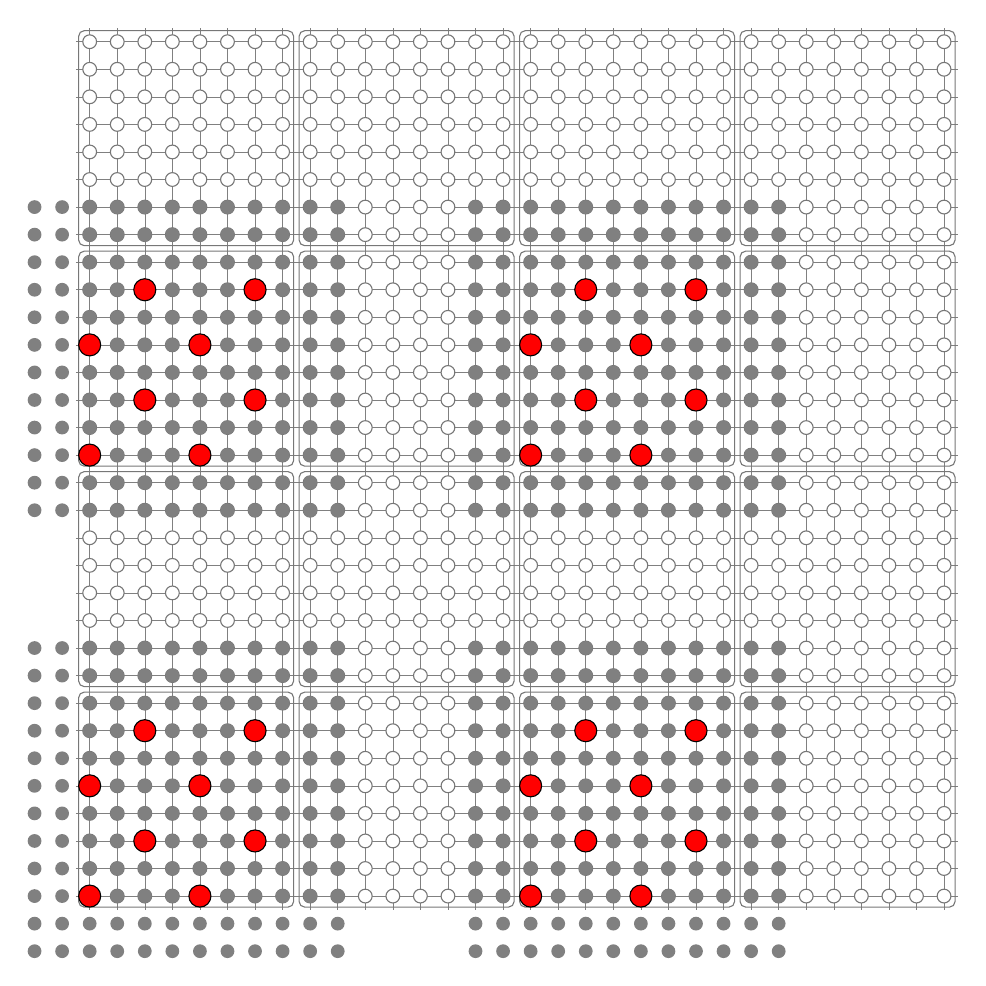
\begin{tikzpicture}[scale=0.35]

\pgfmathtruncatemacro\lcsize{\bksize * \bkcount}
\pgfmathtruncatemacro\lcsizem{\lcsize - 1}
\pgfmathtruncatemacro\lcsizeb{\lcsize - \bksize}


\draw[very thin, gray] (-.5, -.5) grid (\lcsize - .5, \lcsize - .5);

\foreach \x in {0, \bksize, ..., \lcsizeb}
  \foreach \y in {0, \bksize, ..., \lcsizeb} {
    \pgfmathtruncatemacro\n{Mod(\x/\bksize, 2)+2 * Mod(\y/\bksize, 2)+1}
    \draw[colorone, xshift=\x cm, yshift=\y cm, rounded corners=2pt]
      (-.4, -.4) rectangle
      node[red, fill opacity=0, anchor=center, font=\Huge\bfseries\sffamily]
      {\n} (\bksize - .6, \bksize - .6);
  }

\foreach \x in {0, ..., \lcsizem}
  \foreach \y in {0, ..., \lcsizem}{

    \path[draw=colorone, fill=white] (\x, \y) circle(.25);
}


\fillblockgray{0}{0}
\markpartition{0}{0}{0}
\fillblockgray{0}{2}
\markpartition{0}{2}{0}
\fillblockgray{2}{0}
\markpartition{2}{0}{0}
\fillblockgray{2}{2}
\markpartition{2}{2}{0}
\end{tikzpicture}
\end{center}
\caption{\label{fig:blocks}Partition of the lattice into
  blocks.  The sites
marked in gray are loaded into shared memory.}
\end{figure}

To process each point inside a block we also need the neighboring points. We
divide the grid of blocks into subgrids in such a way, that blocks together
with the neighborhood in each subgrid do not overlap (see gray points in
figure~\ref{fig:blocks}). In 2D we need four of such subgrids and eight in 3D
case.

We then start a kernel that process all blocks in one subgrid. Each block in
this subgrid is assigned to a block of $N_{th}$ threads (CTA -- Cooperative
Threads Array). First we fetch the values of the fields from global to shared
memory (including border points see figure~\ref{fig:blocks}). In 3D we use
$B_x=B_y=B_z=16$ which gives altogether $20^3$ field values to be loaded with
additional boundary values on the edges. This gives $32$KB which fits nicely
into 48KB shared memory.

After that each thread updates one site from the first sublattice. This is done
$N_{hit}$ times resulting in what is know as {\em multi-hit} metropolis
algorithm. The advantage is that the corona $c_i$ does not need to be
recalculated again and most of the needed variables resides already in
registers. Then after synchronization, next sublattice is updated and so on.
This whole procedure is repeated $N_{loc}$ times, again taking advantage of the
fact that the field values are already in the shared memory. After that the
kernel writes the shared memory back into global and new kernel is started
processing next subgrid of blocks (see algorithm~\ref{alg:gpu}).

Monte-Carlo calculations require a good source of random numbers. We use the
Tausworthe pseudo--random number generator\cite{howes_thomas07} with one copy
of the generator per thread. The performance could be increased by the use of
simpler generator, but we have not attempted this in this work.

\begin{algorithm}
\begin{algorithmic}[1]
\For{every global sweep}
  \For{every block subgrid}
    \For{every block in subgrid}
      \State load block into shared memory
      \For{every local sublattice}
        \For{every site $i$ in local sublattice}
          \State calculate corona $c_i$
          \For{$k = 1 \dots N_{hit}$}
            \State $\widetilde{\vphi}_i \gets \vphi_i+\eta$
            \State $\Delta H \gets H[\widetilde{\vphi}_i]-H[\vphi_i]$
            \If{$\exp(-\Delta H) > r$}
              \State $\vphi_i \gets \widetilde{\vphi}_i$
            \EndIf
          \EndFor
        \EndFor
        \State \verb!__syncthreads()!
      \EndFor
    \EndFor
  \EndFor
\EndFor
\end{algorithmic}
\caption{\label{alg:gpu} The GPU algorithm. The CPU algorithm differs
  by the absence of the loops over the blocks: lines 2-4.}
\end{algorithm}

One of the problems with lattice simulations is the treatment of the boundary
conditions. The algorithm requires access to the site neighbors during each
update. Index of neighbors can be calculated using simple arithmetic's, except
at the boundaries. Indexing of neighbors requires checking for the boundary at
each update or an expensive modulo operations\footnote{An exception are the
powers of two, where modulo can be cheaply calculated. a general modulo
operation is however quite expensive. }. Another technique is to use the
precalculated and stored indices: for every site we store the index of four or
six nearest neighbors. This is also very flexible but requires a large amount
of memory. This can have a negative impact on the performance and is not well
suitable for the GPU which usually have less RAM then CPU's. In our algorithm
the checking for boundary is needed only when loading to shared memory. Then we
can use simple index arithmetic.

%%%%%%%%%%%%%%%%%%%%%%%%%%%%%%%%%%%%%%%%%%%%%%%%%%%%%%%%%%%%%%%%%%%%%%%%%%%%%%%%

\section[cpu]{CPU implementation\footnote{Source code available at:
\url{https://github.com/ujhpc/phi4}}}

To make a fair comparison with the CPU we have to use both multicore as vector
(SSE/AVX) programming. The parallelization on many cores is relatively easy
using the \emph{OpenMP}. The same restriction apply as on GPU, so we partition
the the lattice in the same way, but we use only one level \emph{i.e.} we do
not partition the lattice into blocks. The SIMD instructions are used to
process four (SSE) or eight (AVX) updates in parallel (similarly to threads on
GPU). At present only portable way to use vector instructions is to use
compiler intrinsic\cite{intr}. In order to avoid obscurity caused by direct of
intrinsics, we have implemented a \emph{"drop-in"} scalar type replacement
class that wraps vector type declared with
\verb!__attribute__((vector_size(N)))! directive and implements missing
operations using intrinsics.

Unfortunately not all scalar \emph{x86} instructions in modern CPUs have vector
counterparts, which is crucial requirement for vectorizing scalar code. In
particular AVX instruction set misses direct vector \emph{XMM/YMM} gather and
scatter instructions (load/save vector register data from/to memory indexed by
other vector register), unlike GPU where gather and scatter is key feature.
This is partially addressed by AVX2, providing masked gather instruction.
Another drawback in lack of 256-bit wide integer operations in AVX, which makes
random number generator utilize 128-bit SSE only, even on 256-bit AVX capable
CPUs. Again this has changed in AVX2, which is unfortunately available only in
\emph{Haswell} desktop processors. Regular \emph{Xeon} server processors need
to wait for an upgrade until next year.

In our CPU implementation we use a small enhancement exploiting the out of
order instruction execution capabilities of the CPU. The most inner loop of the
algorithm looks as follows

\begin{algorithmic}[1]
\For{$n = 1 \dots N_{hit}$}
  \State{calculate $\Delta H$}
  \If{$\mathtt{exp}(-\Delta H) > \mathtt{rand}()$}
    \State accept the move
  \EndIf
\EndFor
\end{algorithmic}

The exponent is an expensive, high latency operation. The processor has to wait
for the $\Delta H$ calculations to finish before it can start the exponent. We
have rewritten this part as

\begin{algorithmic}[1]
\For{$n = 1 \dots N_{hit}$}
  \State $lr \gets \mathtt{log}(\mathtt{rand}())$
  \State{calculate $\Delta H$}
  \If{$-\Delta H > lr$}
    \State accept the move
  \EndIf
\EndFor
\end{algorithmic}

The advantage is now that the argument of \texttt{log} is independent of
$\Delta H$ and the processor is free to reorder the instructions allowing to
hide some of the latency. This implementation is safe even in case when
\texttt{rand()} returns a zero as \texttt{log} then returns \texttt{-Inf}.
Actually the code above is vectorized and calculations of the four or eight
$\log$'s is done in parallel using the \emph{Intel}'s SVML library\cite{svml}.

As already mentioned in the previous section indexing the neighbors can be
quite costly operation requiring expensive modulo operations or large amount of
memory. However if we restrict ourselves to the lattice dimensions that are
powers of two the nearest neighbor calculations can be made using addition and
bitwise operations. This is quite a restrictive approach, not suitable for real
applications but we have decided to use it for comparison with the GPU version.
This is in some respect the ``upper bound'' of the CPU performance.

%%%%%%%%%%%%%%%%%%%%%%%%%%%%%%%%%%%%%%%%%%%%%%%%%%%%%%%%%%%%%%%%%%%%%%%%%%%%%%%%

\section{Performance}
\label{sec:performance}

We have tested our implementations on the following hardware:
\begin{itemize}

\item[GPU] \emph{NVIDIA} GTX 470, 14 \emph{Scalar Multiprocessors}
(448 CUDA cores), 1.2 GHz, \\
CUDA 5.0 Ubuntu Linux 12.04, 1088 Gflops.

\vspace{.5em}

\item[CPU] \emph{Intel} i5-2400S \emph{Sandy Bridge}, 4 core, 2.5 GHz, 12 GB
RAM, \\
OSX 10.8.3, GCC 4.8.0 \verb!-O3! OpenMP, 160 Gflops\footnote{Estimated
according to \cite{intel}, synthetic benchmark available at: \\
\url{https://github.com/ujhpc/flops}}.

\end{itemize}

The overall performance of the algorithm expressed in Gflops or updates per
sec. will depend strongly on the values of the $N_{loc.}$ and $N_{hit}$. The
optimal values of those parameters will depends on the physics of the model in
particular on the values of parameters $\mu^2$, $g$ and $\Lambda$. To describe
the performance in a general way we have decided to fit the execution time $T$
to the following model:

\begin{equation}\label{eq:model}
T  = a+ V \cdot b +
N_{glob.} V \left(c + N_{loc.}\left(d + N_{hit}\cdot e\right)\right) .
\end{equation}
where $V$ is the volume of the lattice.  The interpretation of the
parameters of the model is given in table~\ref{tab:pars-int}.

\begin{table}
\begin{center} \begin{tabular}{lcp{8cm}p{2cm}}
$c$ &--& time per spin needed to load it to shared memory and back.&\\
$d$ &--& time per spin needed to calculate the corona.& 26 ops\\
$e$ &--& time per spin needed to for update including calculation of two
random numbers and exponential. & 64 ops + 1 exp
\end{tabular}
\end{center}
\caption{\label{tab:pars-int}Interpretation of the parameters in the
model~\ref{eq:model}. The last column gives the number of numerical operations
performed by the corresponding step of the algorithm.}
\end{table}

\begin{table}

\begin{center}
\begin{tabular}{|p{4cm}|l|l|l|}\hline\hline
 & float & int  & bit \\\hline
coronas & 26 & & \\\hline
$\Delta H  $ & 13  & & \\\hline
PRNG & 1 & 2  & 21  \\\hline
$\widetilde{\vphi}_i \gets \vphi_i+\eta$& 3 & &\\\hline\hline
\end{tabular}
\end{center}

\caption{\label{tab:instr-count}Number of instructions in different steps of
the algorithm. float -- floating point, int -- integer arithmetic, bit --
shifts and bitwise logical. In the last row we do not include the call to PRNG.
We do not include the instruction needed for indexing.}

\end{table}

The number of updates is given by
\begin{equation}
N_{up} = V \cdot N_{glob.} \cdot N_{loc.} \cdot N_{hit}
\end{equation}
so the time per update is given by
\begin{equation}\begin{split}
\frac{T}{N_{up}} = &
\frac{ a + V \cdot b + N_{glob.}
       V \left(c + N_{loc.}\left(d + N_{hit}\cdot e\right)\right) }
     { V\cdot N_{glob.}\cdot N_{loc.}\cdot N_{hit} }\\
\approx&
\frac{ \left(c + N_{loc.}\left(d + N_{hit}\cdot e\right)\right) }
     { N_{loc.}\cdot N_{hit} }
\end{split}
\end{equation}

Using the data from the table~\ref{tab:pars-int} we obtain that the number of
the operations performed is

\begin{equation}
N_{op} = V\cdot N_{glob.}\cdot N_{loc.}(26+\cdot N_{hit}(64+exp))
\end{equation}
\begin{equation}
  ops =   \frac{ N_op }{ T }
  \approx \frac{ N_{loc.}(26+\cdot N_{hit}(64+exp)) }
               { \left(c + N_{loc.}\left(d + N_{hit}\cdot e\right)\right) }
\end{equation}

We have gathered the data on the execution times of the 3D program for four
different lattice sizes. First thing we noticed is that it is not possible to
fit all the data simultaneously to the model \eqref{eq:model}. However when
fitting data for each lattice size separately we obtain a very good fit
accuracy better then $1\%$ on the average. This is understandable: the
execution time can depend non linearly on the lattice volume. One reason is
that for small lattice sizes not all SM on the GPU are used. For the $64^3$
lattice we need $64^3/128=2048$ threads. With $256$ threads per CTA we use only
$8$ thread blocks, which is much smaller than 14 available SM. Even for $128^3$
lattice the 64 needed blocks will not use the SM evenly. Also the L2 cache may
introduce some non-linear dependence on the lattice size.

The results of the fits are included on the table~\ref{tab:fit}.
\begin{table}
\begin{center}
\begin{tabular}{||r|D{.}{.}{8}|D{.}{.}{8}|D{.}{.}{8}|D{.}{.}{8}||}
\hline\hline
\multicolumn{1}{|c}{$L^3$}
&\multicolumn{1}{|c}{$a+ L^3b$}
&\multicolumn{1}{|c}{$c$}
&\multicolumn{1}{|c}{$d$}
&\multicolumn{1}{|c|}{$e$}\\\hline\hline
GPU &\multicolumn{4}{c||}{} \\\hline
$64^3$  & 0.56  & 1.64e-9   &   2.76e-10  & 1.78e-10 \\
$128^3$ & 0.49  & 1.06e-9   &   2.06e-10  & 1.35e-10 \\
$256^3$ & 0.41  & 9.01e-10  &   1.85e-10  & 1.22e-10 \\
$512^3$ & 0.86  & 6.61e-10  &   2.02e-10  & 1.10e-10 \\ \hline\hline
CPU &\multicolumn{4}{c||}{} \\ \hline
$64^3$  & 0.12  &           &   1.27e-8 &       1.51e-9 \\
$128^3$ & 1.17  &           &   1.34e-8 &       1.45e-9 \\
$256^3$ & 0.93  &           &   1.26e-8 &       1.43e-9 \\
$512^3$ & 3.72  &           &   1.35e-8 &       1.44e-9 \\ \hline\hline
\end{tabular}
\end{center}
\caption{\label{tab:fit}Results of the fit of the formula \eqref{eq:model} GPU
and \eqref{eq:model-cpu} CPU.}
\end{table}
In case of CPU as we do not loop over the blocks the model is:
\begin{equation}\label{eq:model-cpu}
T  = a+ V \cdot b +
N_{glob.} V \left(d + N_{hit}\cdot e\right).
\end{equation}

The coefficient $d$ is the time per spin needed to load it from and to memory
together with the calculation of the corona. The time per update in this case
is given by:

\begin{equation}\begin{split}
\frac{T}{N_{up}}=&\frac{a+ V \cdot b + N_{glob.} V \left(d + N_{hit}\cdot e\right)}{V\cdot N_{glob.}\cdot N_{hit}}\\
\approx&
\frac{d + N_{hit}\cdot e}{\cdot N_{hit}}
\end{split}
\end{equation}
and
\begin{equation}
ops\approx \frac{ 26+N_{hit}(64+exp)}{ \left(d + N_{hit}\cdot e\right)}
\end{equation}
\begin{table}
\begin{center}
\begin{tabular}{|r|rrr|rrr|c|}
\hline\hline
\multicolumn{1}{|}{} & \multicolumn{3}{c|}{GPU}
                     & \multicolumn{3}{c|}{CPU}
                     & GPU/CPU\\\hline
\multicolumn{1}{|c}{size} &
\multicolumn{1}{|c|}{ns} &
\multicolumn{1}{c|}{Gops} &
\multicolumn{1}{c|}{Gexp/s} &
\multicolumn{1}{c|}{ns} &
\multicolumn{1}{|c}{Gops} &
\multicolumn{1}{|c|}{Glog/s} &
speedup \\ \hline\hline
$128^3$ & 0.16 & 412 & 6.1 & 3.1 & 21.4 & 0.32 & $19\times$ \\ \hline
$256^3$ & 0.15 & 456 & 6.8 & 3.1 & 21.8 & 0.32 & $20\times$ \\ \hline
$512^3$ & 0.14 & 490 & 7.3 & 3.1 & 21.6 & 0.32 & $22\times$ \\ \hline\hline
\end{tabular}

\end{center}
\caption{\label{tab:comp} Performance of the algorithm.}
\end{table}

\subsection{GPU cache}

The good performance of the presented GPU algorithm comes from the effective
use of the shared memory. We have also checked to which extend this could be
achieved by just using the automatic cache capabilities of modern GPU's. To
this end we have implemented a version of the algorithm which did not use the
shared memory, however the access pattern was the same. The idea was that the
first iteration of the local sweep loop would fill the L1 cache and consecutive
iterations would not need to access the global memory and the performance
should be comparable to our original implementation.

This turned out not to be the case. The algorithm using the L1 cache was
approximately six times slower than the one using shared memory. This
deteriorated performance could be traced back to large number of cache misses.
Nominally the $20^3$ block should fit in L1 cache as it did fit into the shared
memory. However the cache line is 32 words long (128B) and the blocks are not
aligned on the cache lines boundaries (see gray points on the
figure~\ref{fig:blocks}). On top of that the cache is probably not fully
associative. All that together implies that the cache size should be up to four
or five times bigger to accommodate the whole block.

%%%%%%%%%%%%%%%%%%%%%%%%%%%%%%%%%%%%%%%%%%%%%%%%%%%%%%%%%%%%%%%%%%%%%%%%%%%%%%%%

\section{Extensions and limitations}

The above implementation can be easily adapted to other variants of the model.
The $\Delta H$ can be arbitrary within the constraints that it cannot access
points outside of the neighborhood considered in this contribution. Of course
when the $\Delta H$ calculation requires smaller number of lattice points the
above procedure can be overly complicated and thus not optimal. In that case it
may be advantageous to use \eg the checkerboard decomposition.

%%%%%%%%%%%%%%%%%%%%%%%%%%%%%%%%%%%%%%%%%%%%%%%%%%%%%%%%%%%%%%%%%%%%%%%%%%%%%%%%

\section{Discussion}

Results presented in table~\ref{tab:comp} show clear advantage of the GPU over
CPU. This is hardly surprising, but the $20\times$ difference is much higher
than comes from comparison of theoretical performance ratio of tested i5 CPU to
\emph{GTX 470} equal $8\times$. The GTX is thus more efficient in that sense
that is capable of achieving performance much closer to the peak. This can be
attributed to two main reasons:

\begin{itemize}

\item The shared memory that acts as an managed cache allows to use the small
cache size much more effectively. In particular it is possible on the GPU to
fit the whole $20^3$ grid block into the shared memory. This is not possible
using the conventional cache both on GPU and CPU leading to large number of
cache misses and decrease of performance.

\item Modern CPU are not fully vector processors. Not every scalar instruction
has a vector counterpart. In particular the eight words wide integer
instructions are present in AVX2 instruction set, not available to \emph{Xeon}
server CPUs, which has impact on pseudo-random number generator using only
128-bit wide AVX instructions.

\item Efficient load and store vector (gather/scatter) instruction are also
missing in AVX. When not loading/storing from the consecutive memory location
they are effectively serialized into scalar loads/stores. On top of this GPUs
provide enormous memory bandwidth comparing to CPU.

These however are not being accounted in raw \emph{Gops} and \emph{Glogs}
calculations above.

\item GPUs provide hardware exponent, \emph{i.e.} our \emph{GTX 470} can
execute 4 exponent operations in single cycle of \emph{Scalar Multiprocessor}
and recent GPUs can execute 8 exponent in single cycle. CPUs do not provide
efficient hardware exponent implementation. Fastest AVX
implementations\cite{svml} need minimum 20 CPU cycles, however there is no
single implementation that works best for all \emph{x86} CPUs\cite{nolib}.

\item CPUs have less general purpose registers than GPUs, making CPU code more
prone to latency problems caused by tight register dependencies. Peak
performance can be reached only by synthetic benchmarks, while real computation
algorithms seldom reach half of it.

\end{itemize}

Undeniably the trend of vectorization of CPUs is continuing and the software
that wants to stay competitive must adapt to it. However, the current CPU make
this more difficult than the GPU, due to the lack of some crucial vector
features present on GPU, incomplete vectorization support provided by compilers
and complicated programming model.

The CPU manufacturers are are trying to address these issues. \emph{Intel Xeon
Phi} has a extended 512-bit wide vector instruction set with hardware
gather/scatter, also recently released \emph{Haswell} CPU architecture with
AVX2 instruction set contains 256-bit wide integer operations and gather
instructions. AVX2 gather is still however internally mapped to several
$\mu$-ops, yet it provides clear benefits in terms of instruction number
reduction having notable impact on performance.

We already have some preliminary results that show $1.5\times$ performance
boost making or CPU implementation utilize some of new AVX2 instructions. We
are also working to port our code to recent NVIDIA \emph{Kepler} architecture
and \emph{Xeon Phi} accelerator.

%%%%%%%%%%%%%%%%%%%%%%%%%%%%%%%%%%%%%%%%%%%%%%%%%%%%%%%%%%%%%%%%%%%%%%%%%%%%%%%%

\begin{thebibliography}{9}

\bibitem{top500} \url{http://www.top500.org/}

\bibitem{spin1} Benjamin Block , Peter Virnau , Tobias Preis, Computer Physics
Communications, Volume 181 (2010) 1549–1556.

\bibitem{spin2} Ezequiel E. Ferrero, Juan Pablo De Francesco, Nicolás Wolovick,
Sergio A. Cannas. Computer Physics Communications, volume 183, 1578--1587, 2012

\bibitem{Checkboard}B.~Block, P.~Virnau, T.~Preis ``Multi-GPU Accelerated
Multi-Spin Monte Carlo Simulations of the 2D Ising Model''. Computer Physics
Communications, Volume 181, 1549--1556,2010

\bibitem{weigel} M.~Weigel, J. Comput. Phys. \textbf{231},  (2012) 3064.

\bibitem{parisi} G.~Parisi ``Statistical Field Theory'' Chapter 5, Perseus
Books Publishing (1998).

\bibitem{metropolis} N.~Metropolis, A.W.~Rosenbluth, M.N.~Rosenbluth,
A.H.~Teller, E. Teller, J.~Chem.~Phys.~\textbf{21} (6) (1953) 1087--1092.

\bibitem{binney} J.J.~Binney, N.J. Dowrick, A.J.~Fisher, and M.E.J.~Newman
``The Theory of Critical Phenomena'', Oxford University Press (1993).

\bibitem{Fermi} ``NVIDIA's Next Generation CUDA ComputeArchitecture: Fermi'' \\
\url{http://www.nvidia.com/content/PDF/fermi_white_papers/NVIDIA_Fermi_Compute_Architecture_Whitepaper.pdf}

\bibitem{howes_thomas07} Lee Howes and David Thomas. ``{\em Efficient random
number generation and application using {CUDA}.}'' In Hubert Nguyen, editor,
{\em GPU Gems 3}, chapter~37. Addison Wesley, August 2007.

\bibitem{intel} ``Intel 64 and IA-32 Architectures Software Developer Manuals''
\\
\url{http://www.intel.com/content/www/us/en/processors/architectures-software-developer-manuals.html}

\bibitem{intr} ``Intel C++ Intrinsic Reference.'' \\
\url{http://software.intel.com/file/18072/} \\
``Intel Intrinsics Guide'' \\
\url{http://software.intel.com/en-us/articles/intel-intrinsics-guide}

\bibitem{svml} ``Overview: Intrinsics for Short Vector Math Library (SVML)
Functions'' \\ \url{http://software.intel.com/en-us/node/462496}

\bibitem{nolib} Agner Fog ``Still no library that is optimal on all
processors'' \\ \url{http://www.agner.org/optimize/blog/read.php?i=209&v=t}

\end{thebibliography}

\end{document}
